\chapter{Simple Machines}

As mentioned earlier, physicists define work as the force applied times the distance over which it is applied. For example, if you push your car 100 meters with a force of 17 newtons, you have done 1700 joules of work.

Humans have long needed to move heavy objects, so many centuries ago, we developed simple machines to reduce the amount of force necessary to perform such tasks. These include:

\begin{itemize}
    \item Levers
    \item Pulleys
    \item Inclined planes
    \item Gears
    \item Hydraulics
    \item Screws
\end{itemize}

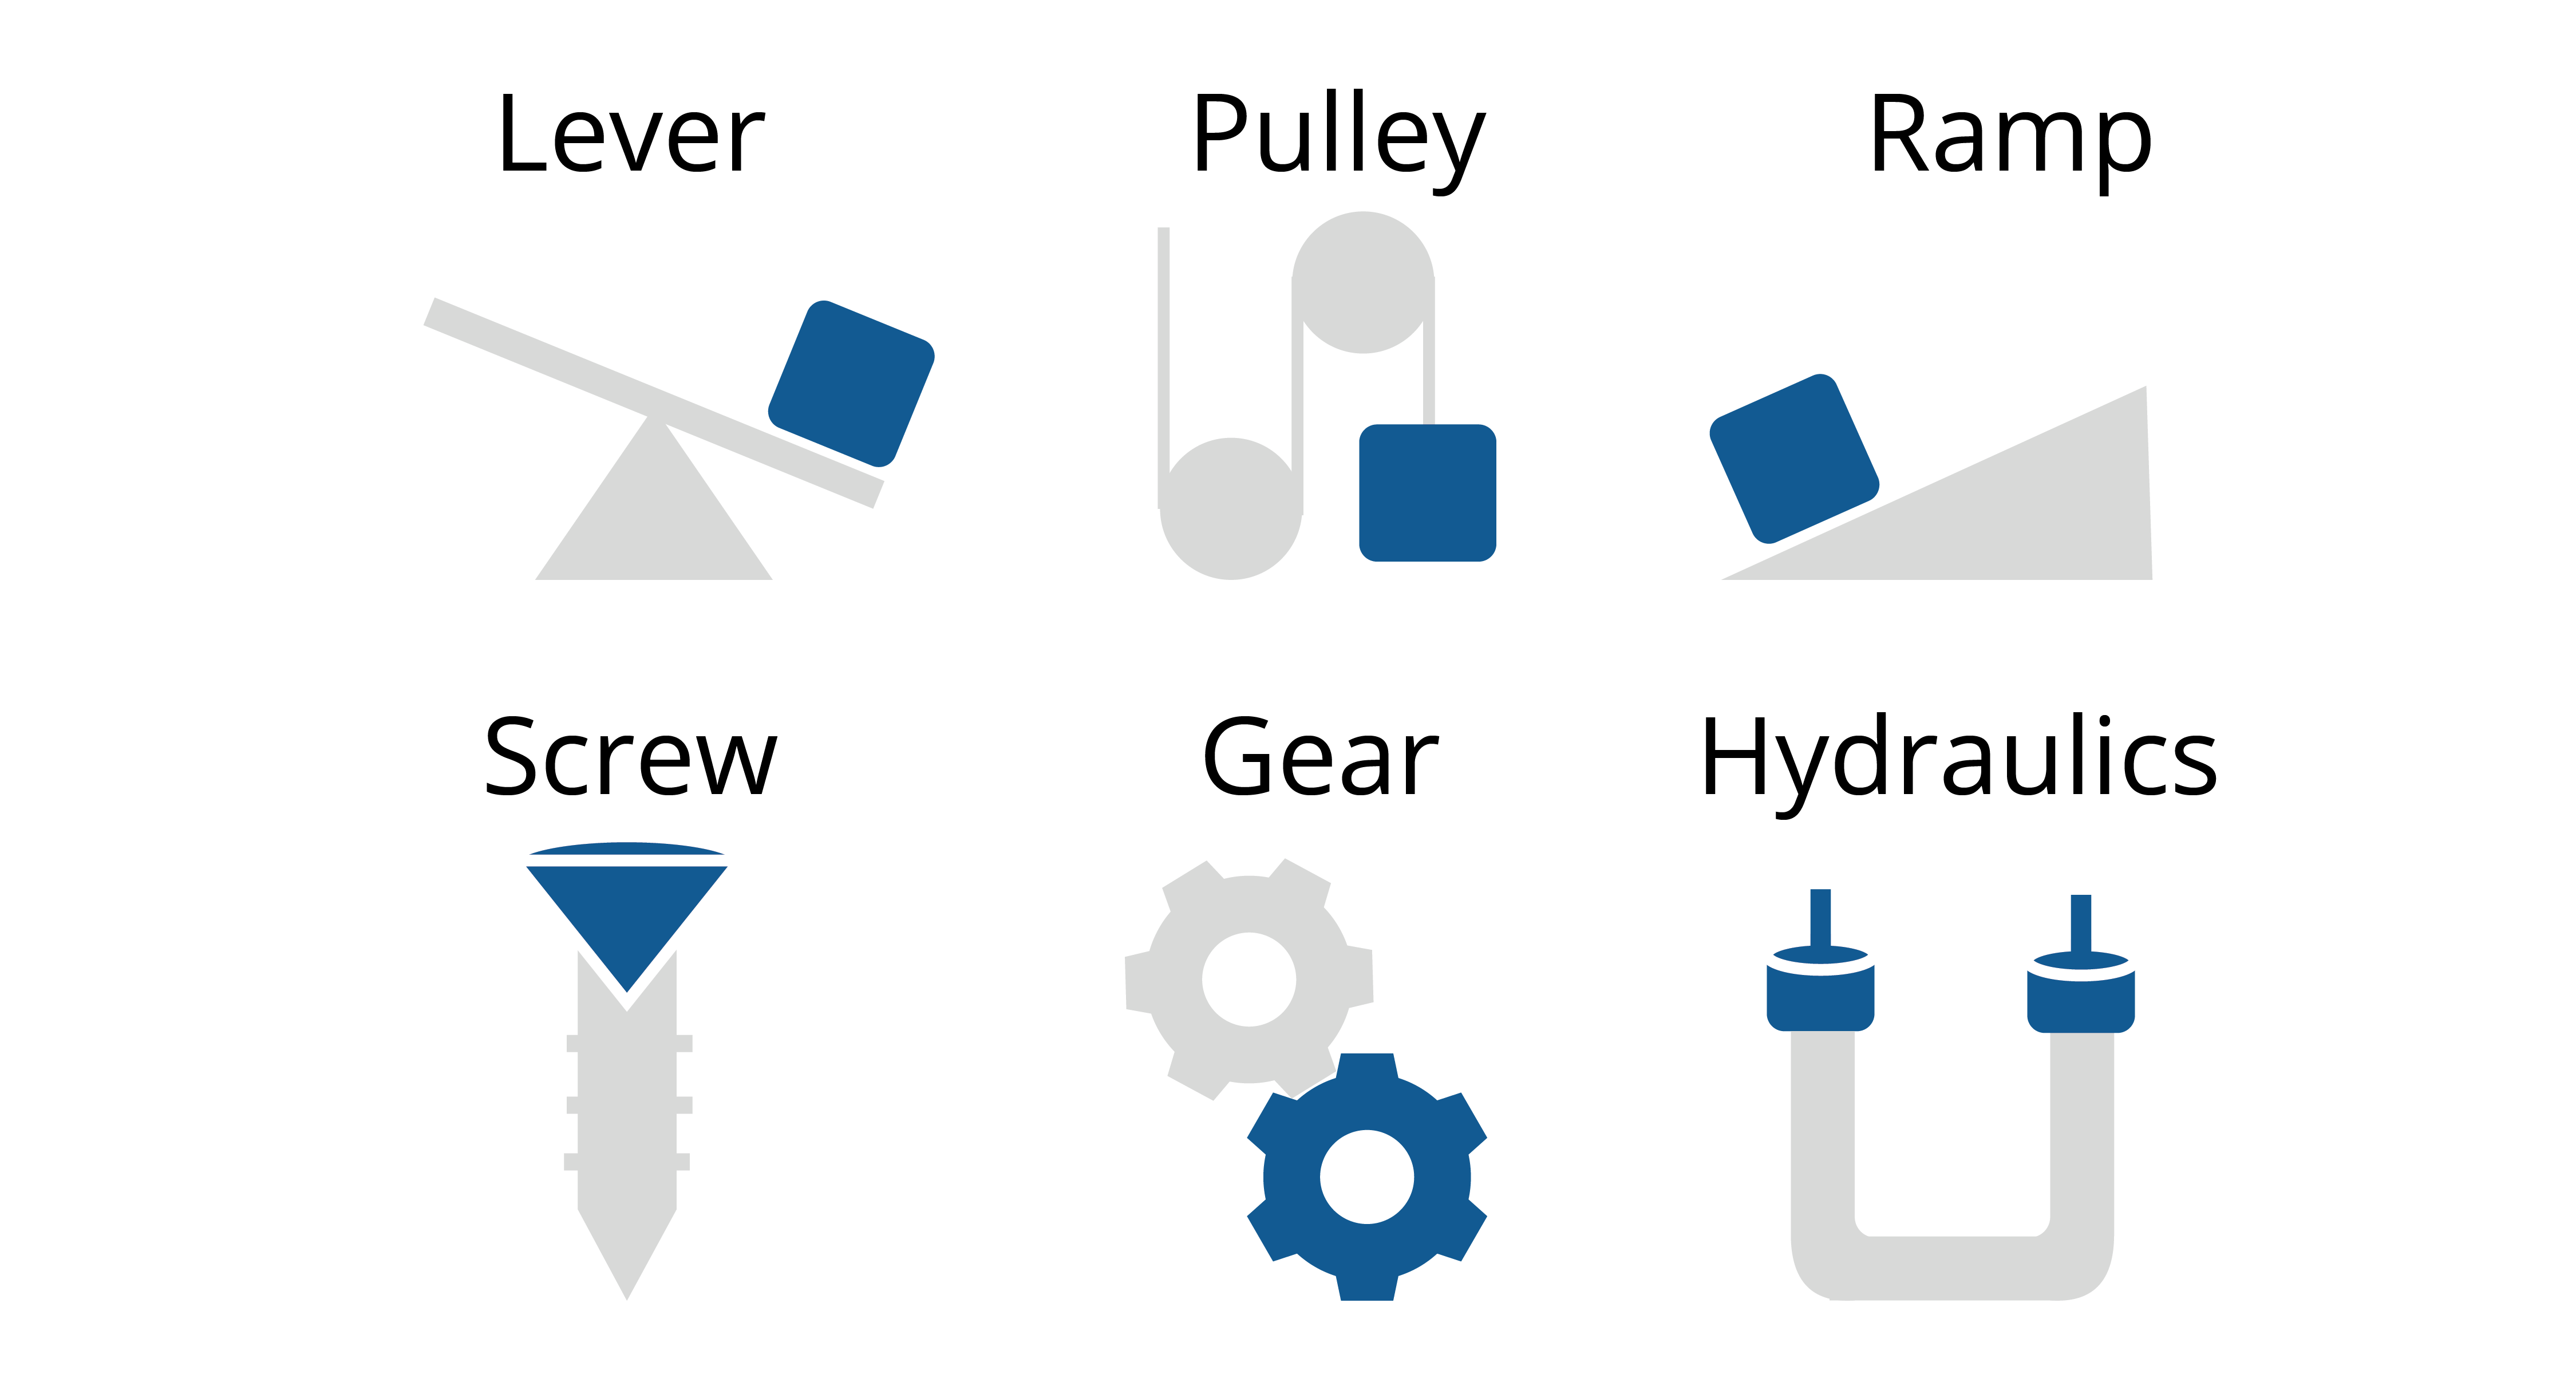
\includegraphics[width=\textwidth]{simplemachines.png}

While these machines can reduce the force needed, they do not change the total amount of work that must be done. For instance, if the force is reduced by a factor of three, the distance over which the force must be applied increases by the same factor.

The term \textit{mechanical advantage} refers to the increase in force achieved by using these machines.

\section{Levers}

A lever pivots on a fulcrum. To decrease the necessary force, the load is placed closer to the fulcrum than where the force is applied.

Physicists also discuss the concept of \newterm{torque} created by a force. When you apply force to a lever, the torque is the product of the force you exert and the distance from the point of rotation.

Torque is typically measured in newton-meters.

To balance two torques, the products of force and distance must be equal. Thus, assuming the forces are applied in the correct direction, the equation becomes:

\[
R_L F_L = R_A F_A
\]

where \( R_L \) and \( R_A \) represent the distances from the fulcrum to where the load’s force and the applied force are exerted, respectively, and \( F_L \) and \( F_A \) are the magnitudes of the forces.

\begin{Exercise}[title={Lever}, label=lever]
Paul, who weighs 70 kilograms, sits on a see-saw 4 meters from the fulcrum. Jan, who weighs 50 kilograms, wishes to balance the see-saw. How far should Jan sit from the fulcrum?
\end{Exercise}
\begin{Answer}[ref=lever]
Paul exerts a force of \( 70 \times 9.8 = 686 \) newtons at a distance of 4 meters from the fulcrum, creating a torque of \( 686 \times 4 = 2744 \) newton-meters. Jan exerts a force of \( 50 \times 9.8 = 490 \) newtons.

Let \( r \) be the distance from the fulcrum to Jan's seat. To balance the torques:

\[
490 \times r = 2744
\]

Solving for \( r \), we find \( r = \frac{2744}{490} \approx 5.6 \) meters.
\end{Answer}

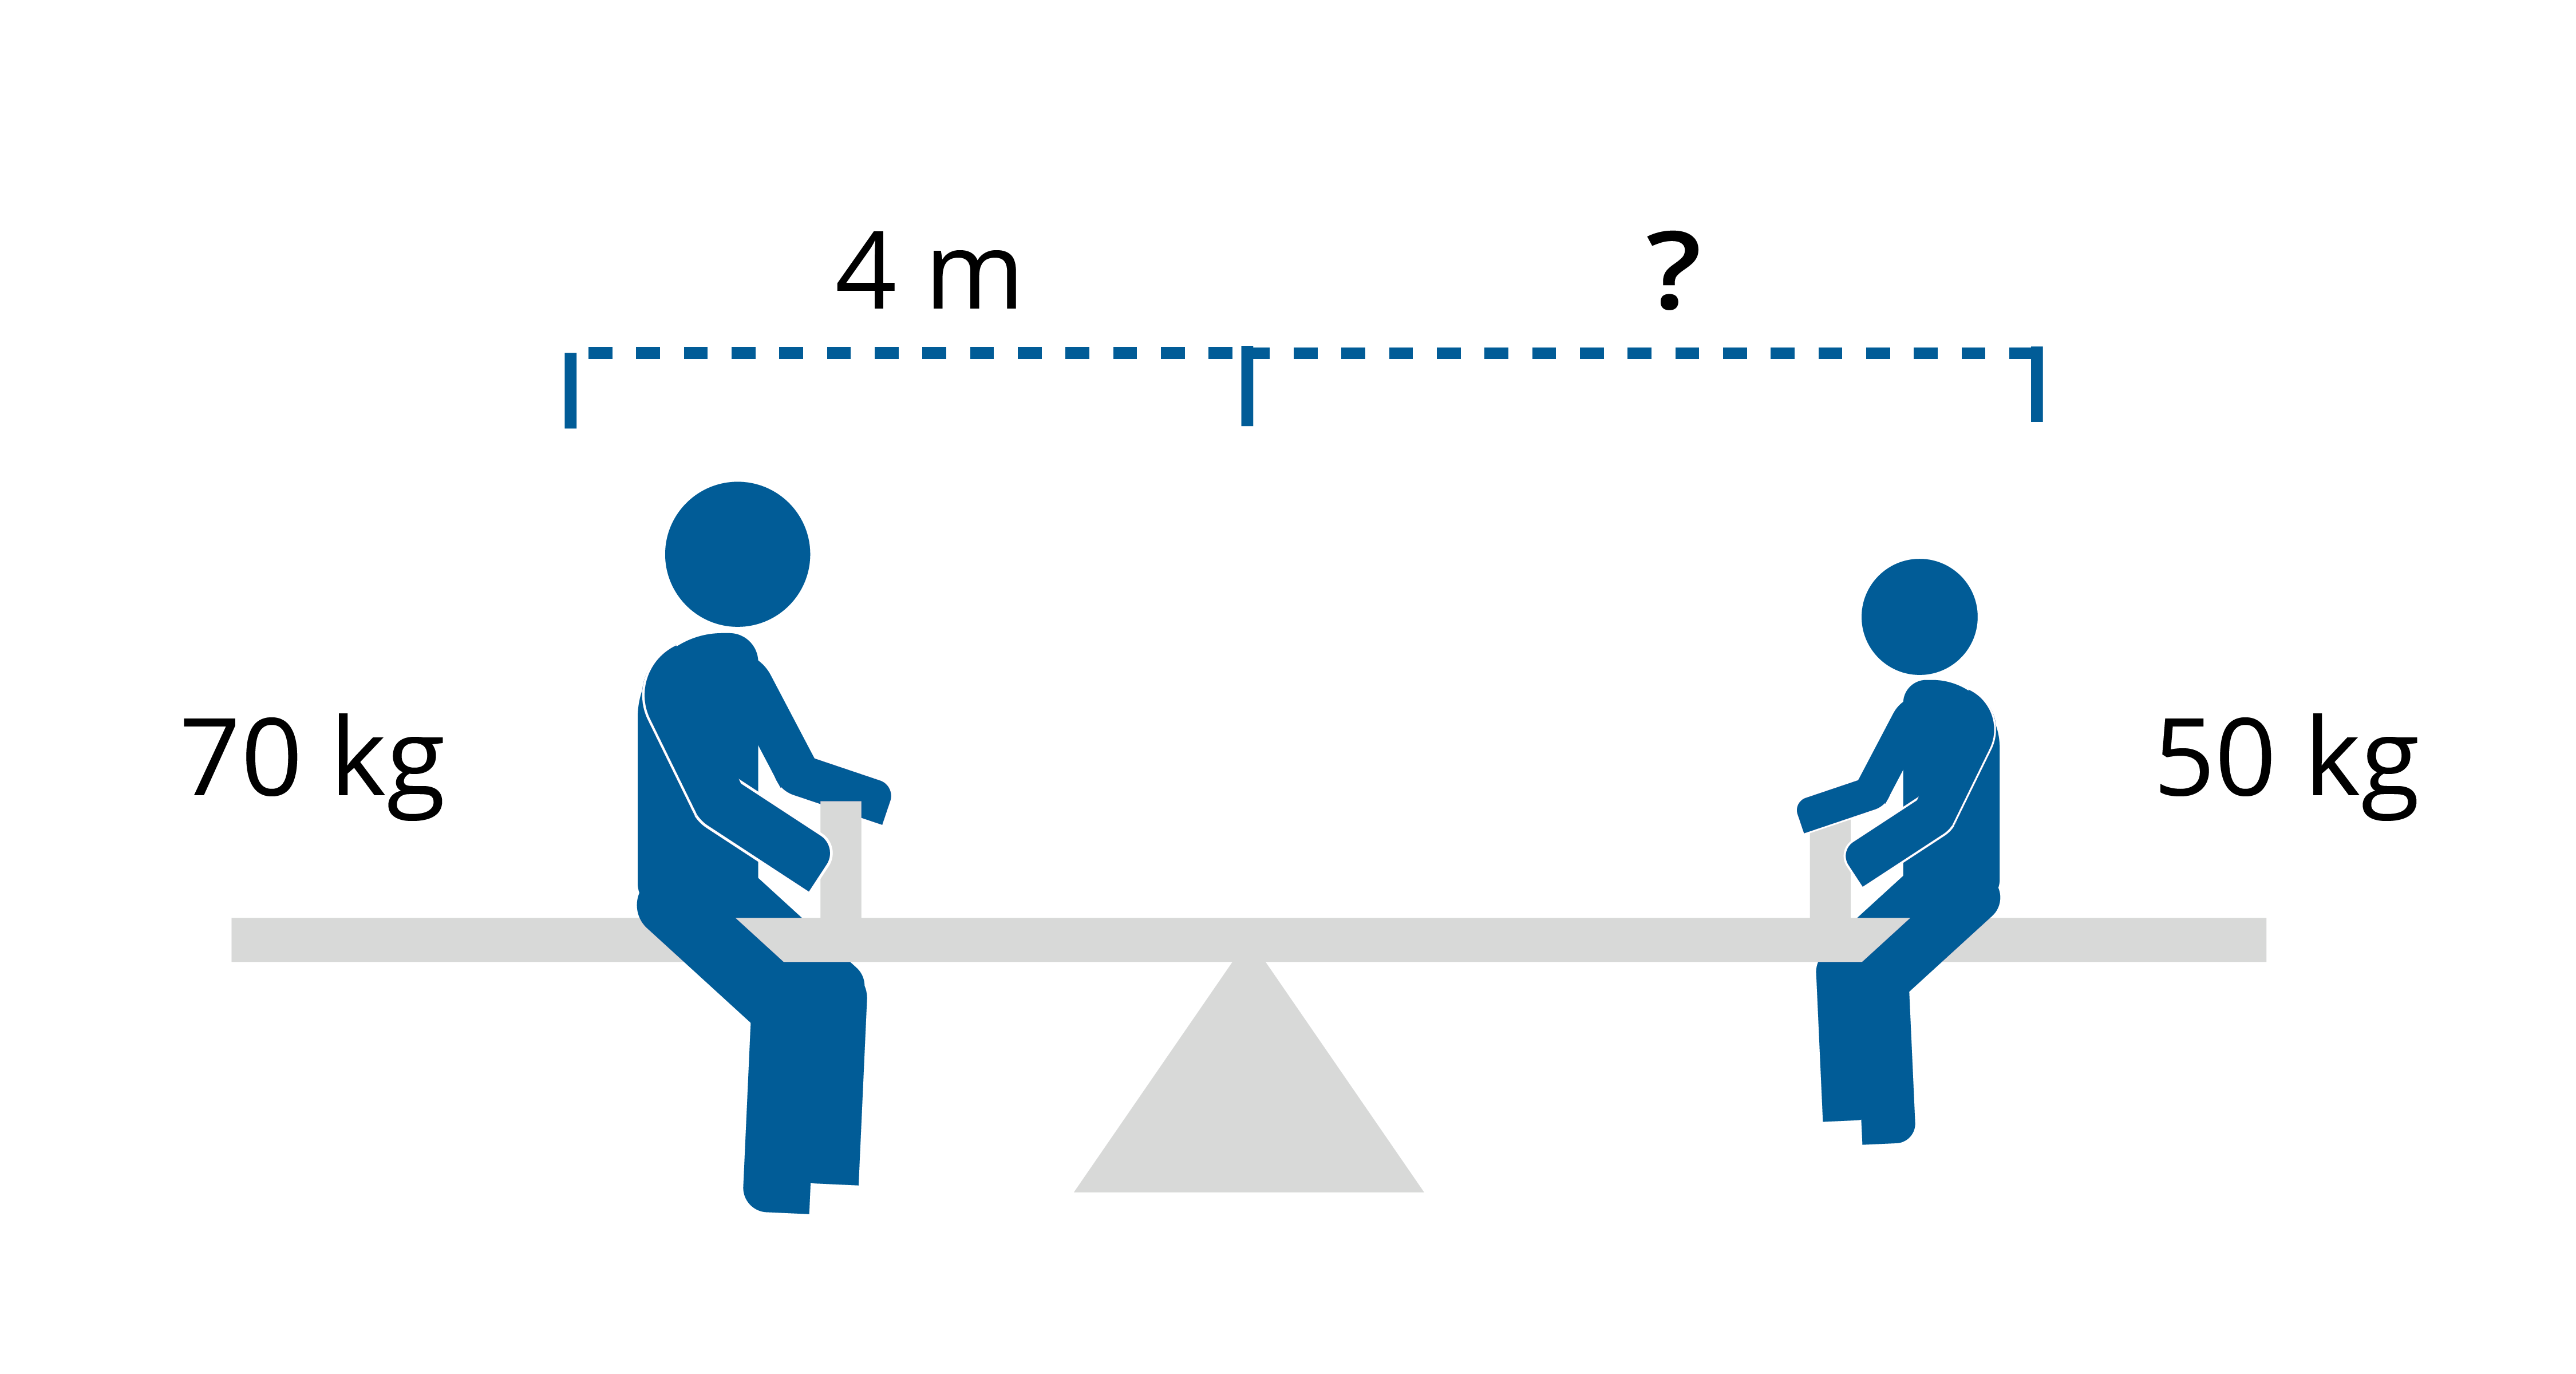
\includegraphics[width=0.6\textwidth]{seesaw.png}

\section{Inclined Planes}

Inclined planes, or ramps, allow you to roll or slide objects to a higher level. Steeper ramps require less mechanical advantage. For instance, it is much easier to roll a ball up a wheelchair ramp than a skateboard ramp.

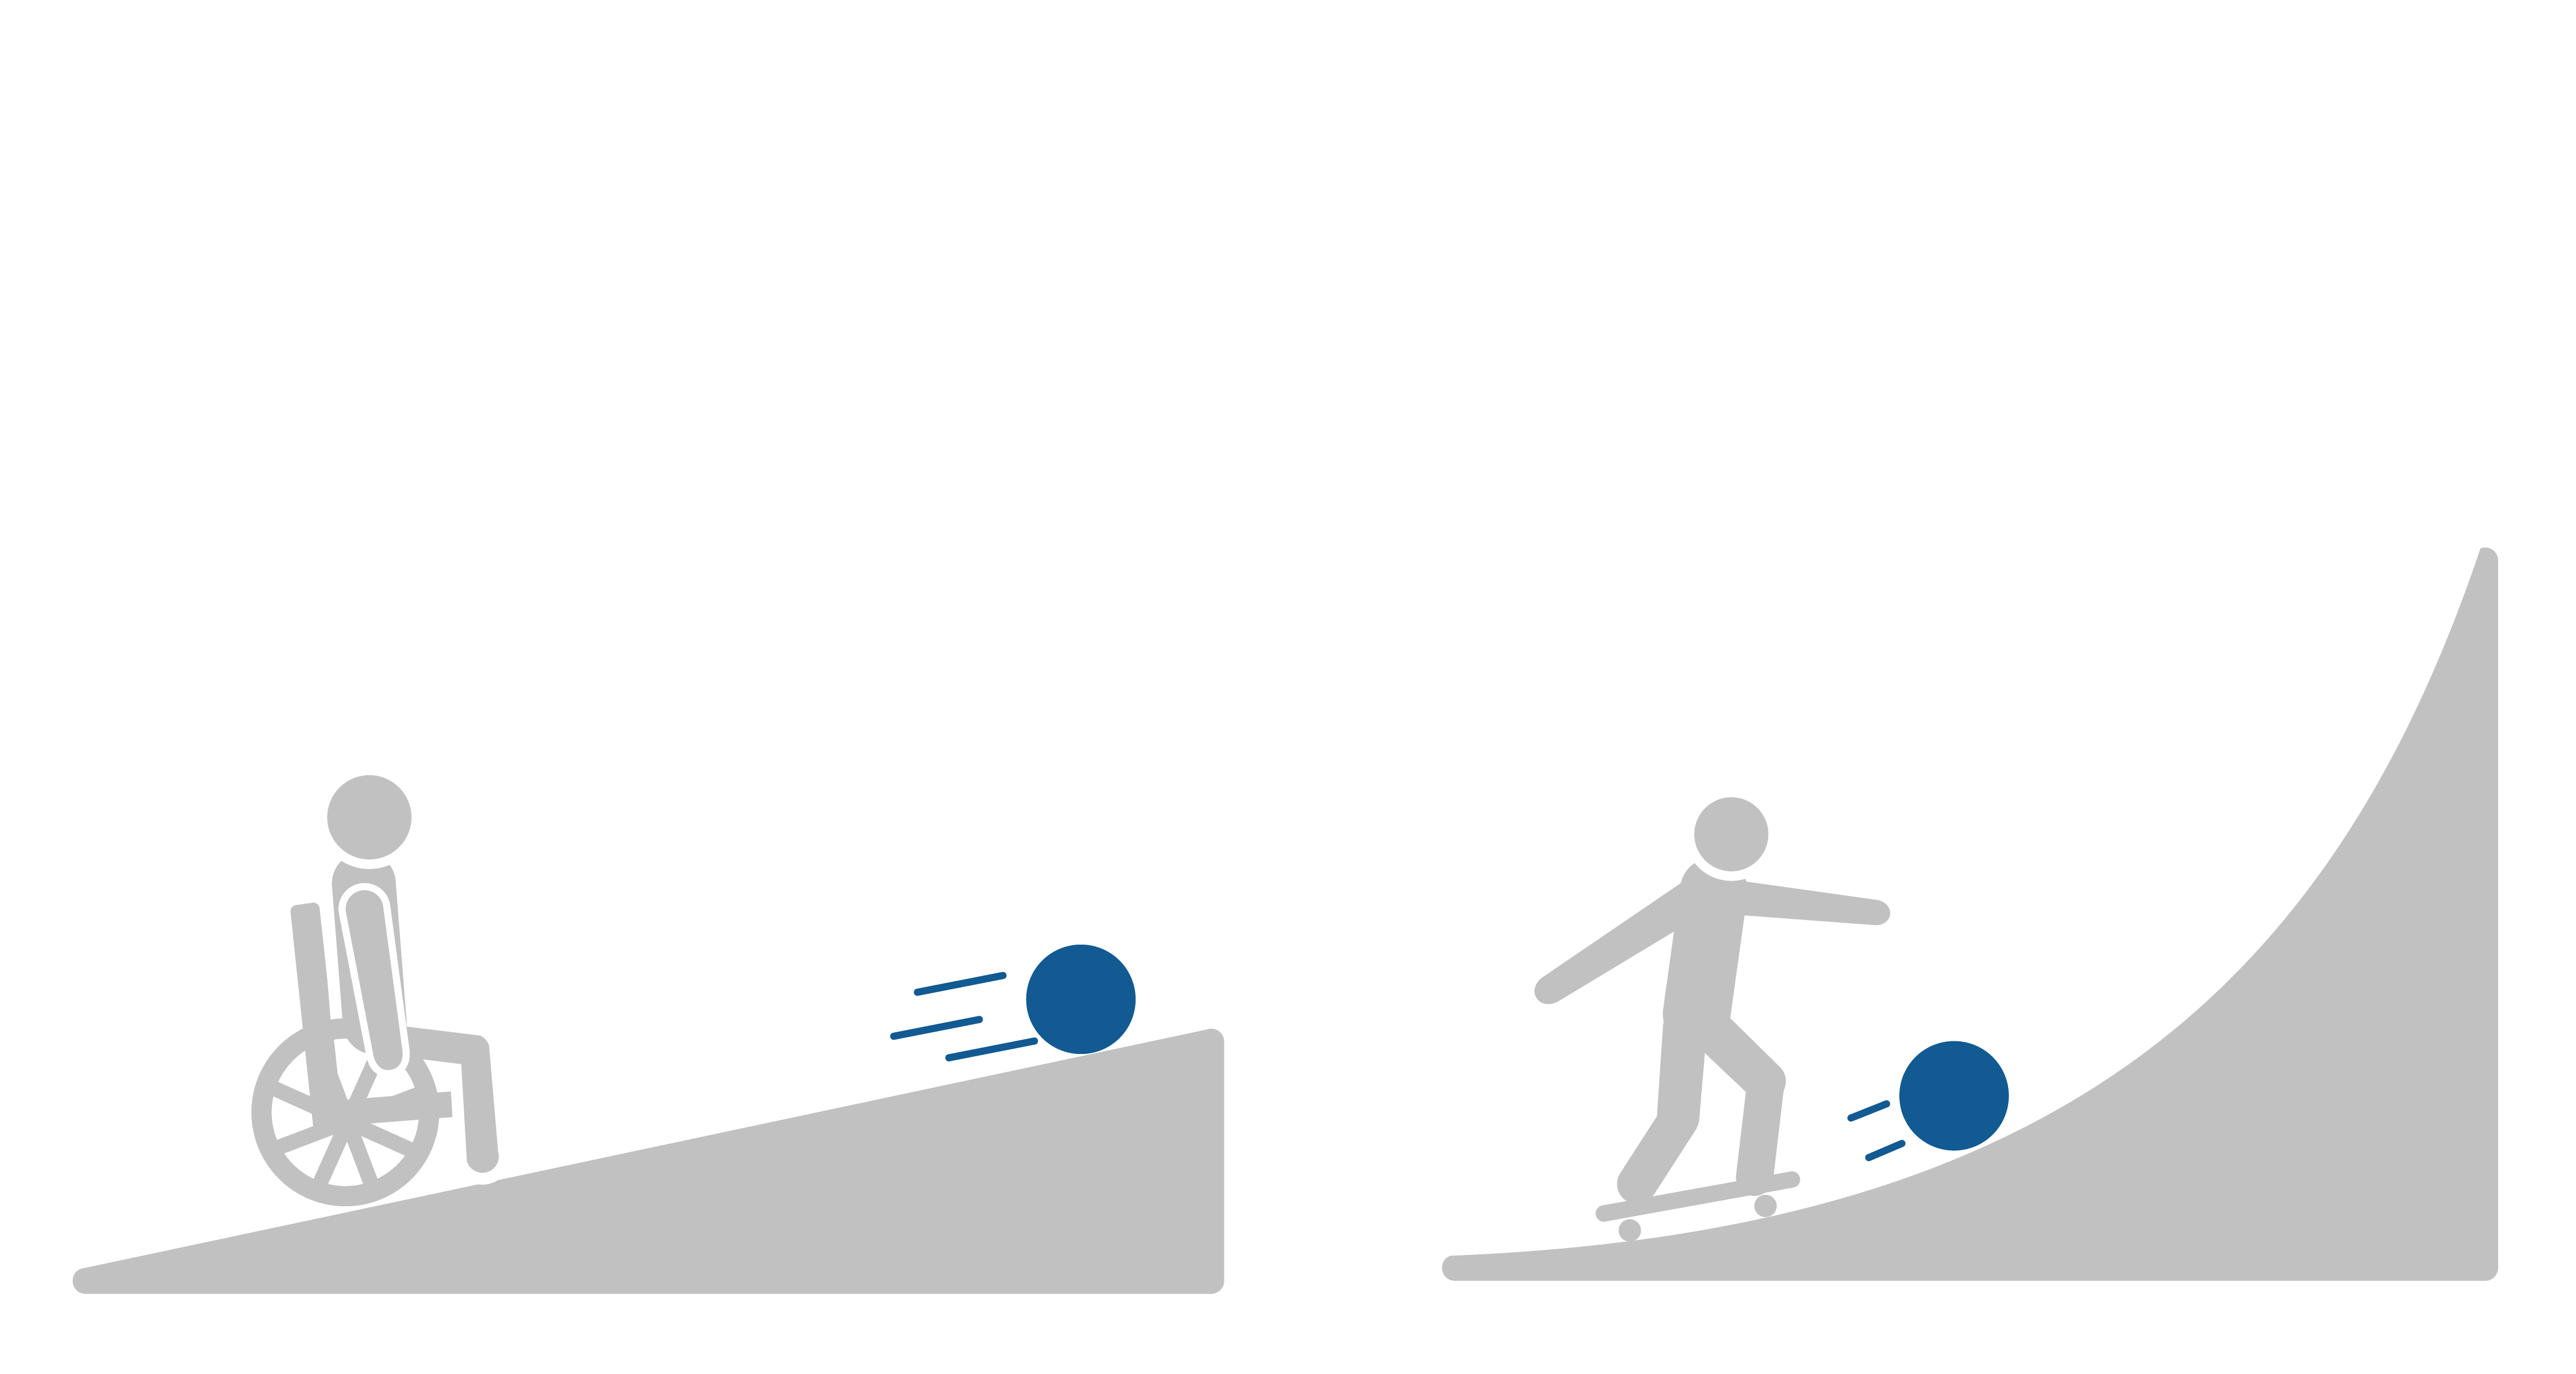
\includegraphics[width=\textwidth]{rampcomparison.png}

Assuming the incline has a constant steepness, the mechanical advantage is equal to the ratio of the length of the inclined plane to the height it rises.

If friction is neglected, the force required to push a weight up the inclined plane is given by:

\[
F_A = \frac{V}{L} F_G
\]

where \( F_A \) is the applied force, \( L \) is the length of the inclined plane, \( V \) is the vertical rise, and \( F_G \) is the gravitational force acting on the mass.

(We will discuss sine function later, but in case you're familiar with it, note that:

\[
\frac{V}{L} = \sin{\theta}
\]

where \( \theta \) is the angle between the inclined plane and the horizontal surface.)

\begin{Exercise}[title={Ramp}, label=ramp]
A barrel of oil weighs 136 kilograms. You can apply a force of up to 300 newtons. You need to get the barrel onto a platform that is 2 meters high. What is the shortest length of inclined plane you can use?
\end{Exercise}
\begin{Answer}[ref=ramp]
The weight of the barrel is \( 136 \times 9.8 = 1332.8 \) newtons.

Let \( L \) be the length of the inclined plane. The force needed to push the barrel up is related by:

\[
300 = \frac{2}{L} \times 1332.8
\]

Solving for \( L \), we find \( L = \frac{2 \times 1332.8}{300} \approx 8.885 \) meters.
\end{Answer}

\section{Gears}

Gears have teeth that mesh with each other. When you apply torque to one gear, it transfers torque to the other. The resulting torque is increased or decreased depending on the ratio of the number of teeth on the gears.

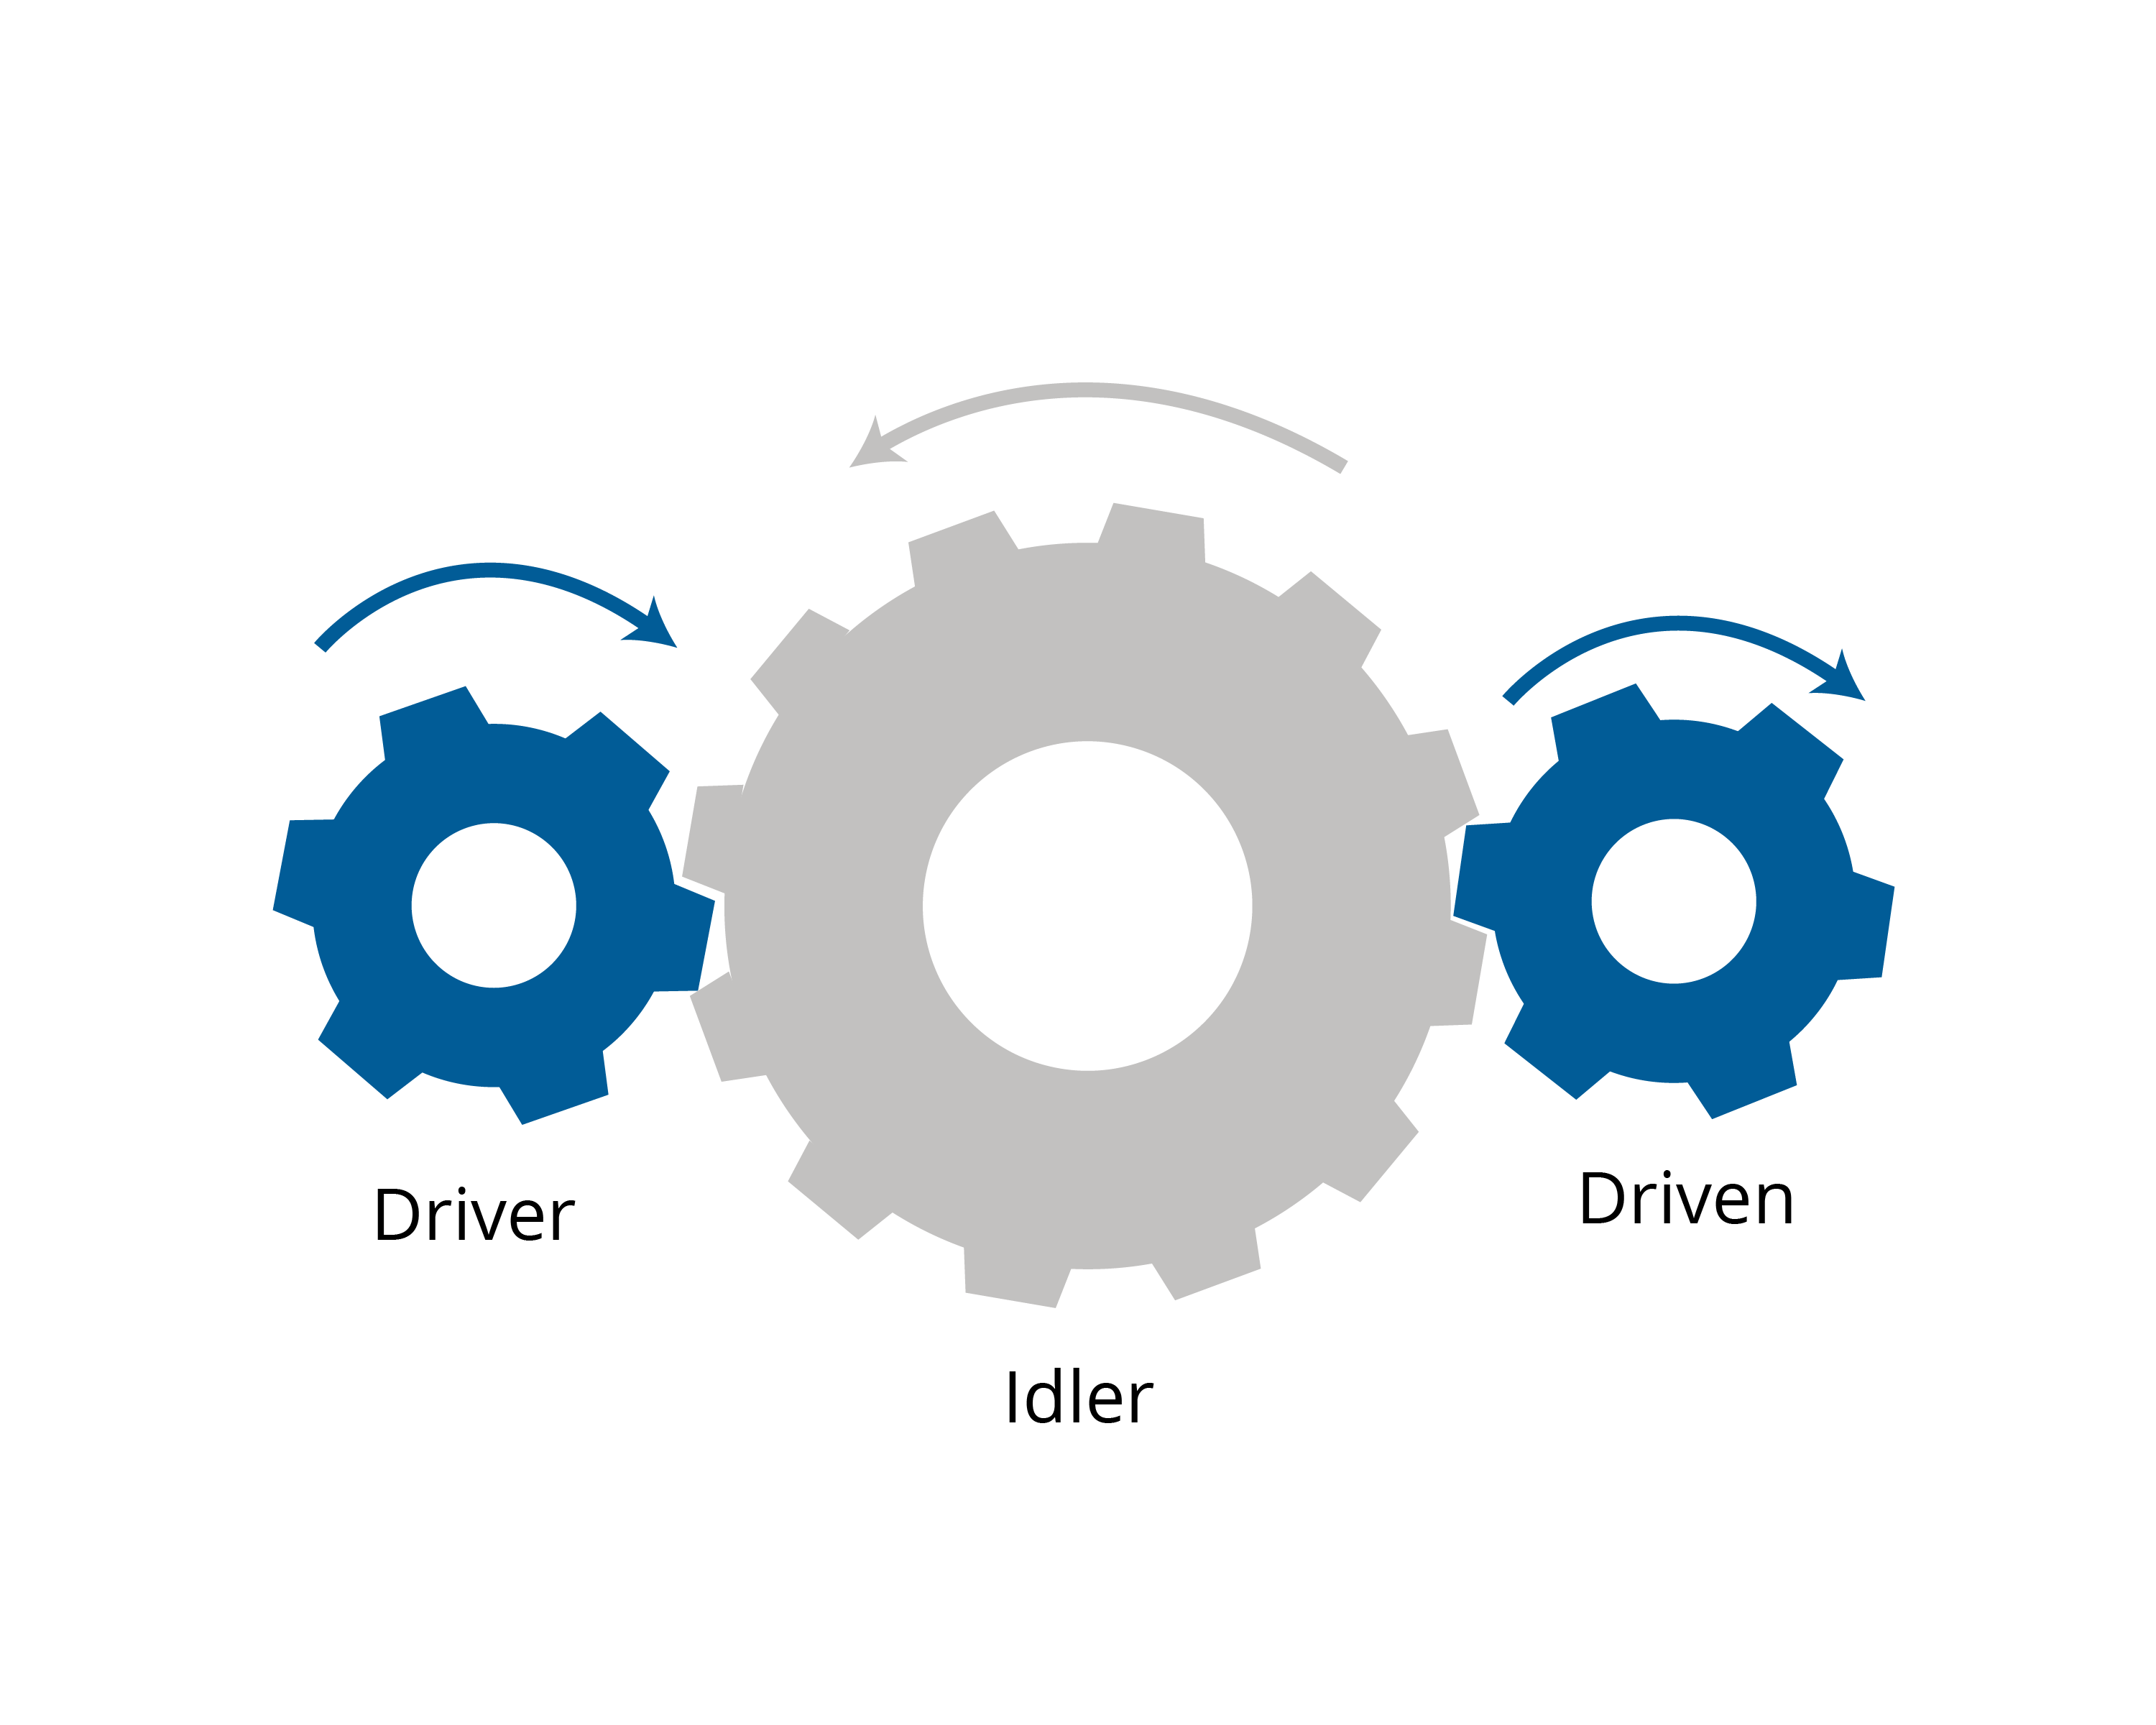
\includegraphics[width=0.7\textwidth]{gearsNew.png}

If \( N_A \) is the number of teeth on the gear you are turning with a torque of \( T_A \), and \( N_L \) is the number of teeth on the gear it is turning, the resulting torque is:

\[
T_L = \frac{N_A}{N_L} T_A
\]

\begin{Exercise}[title={Gears}, label=gear]
In a bicycle, the goal is not always to gain mechanical advantage, but to spin the pedals slower while applying more force.

You like to pedal your bike at 70 revolutions per minute. The chainring connected to your pedals has 53 teeth. The circumference of your tire is 2.2 meters. You want to ride at 583 meters per minute.

How many teeth should the rear sprocket have?
\end{Exercise}
\begin{Answer}[ref=gear]
The equation relating these quantities is:

\[
583 = 70 \times 2.2 \times \frac{53}{n}
\]

Solving for \( n \), we find \( n = 14 \) teeth.
\end{Answer}

\section{Hydraulics}

In a hydraulic system, such as a car's braking system, you exert force on a piston filled with fluid. The fluid transmits this pressure into another cylinder, where it pushes yet another piston that moves the load.

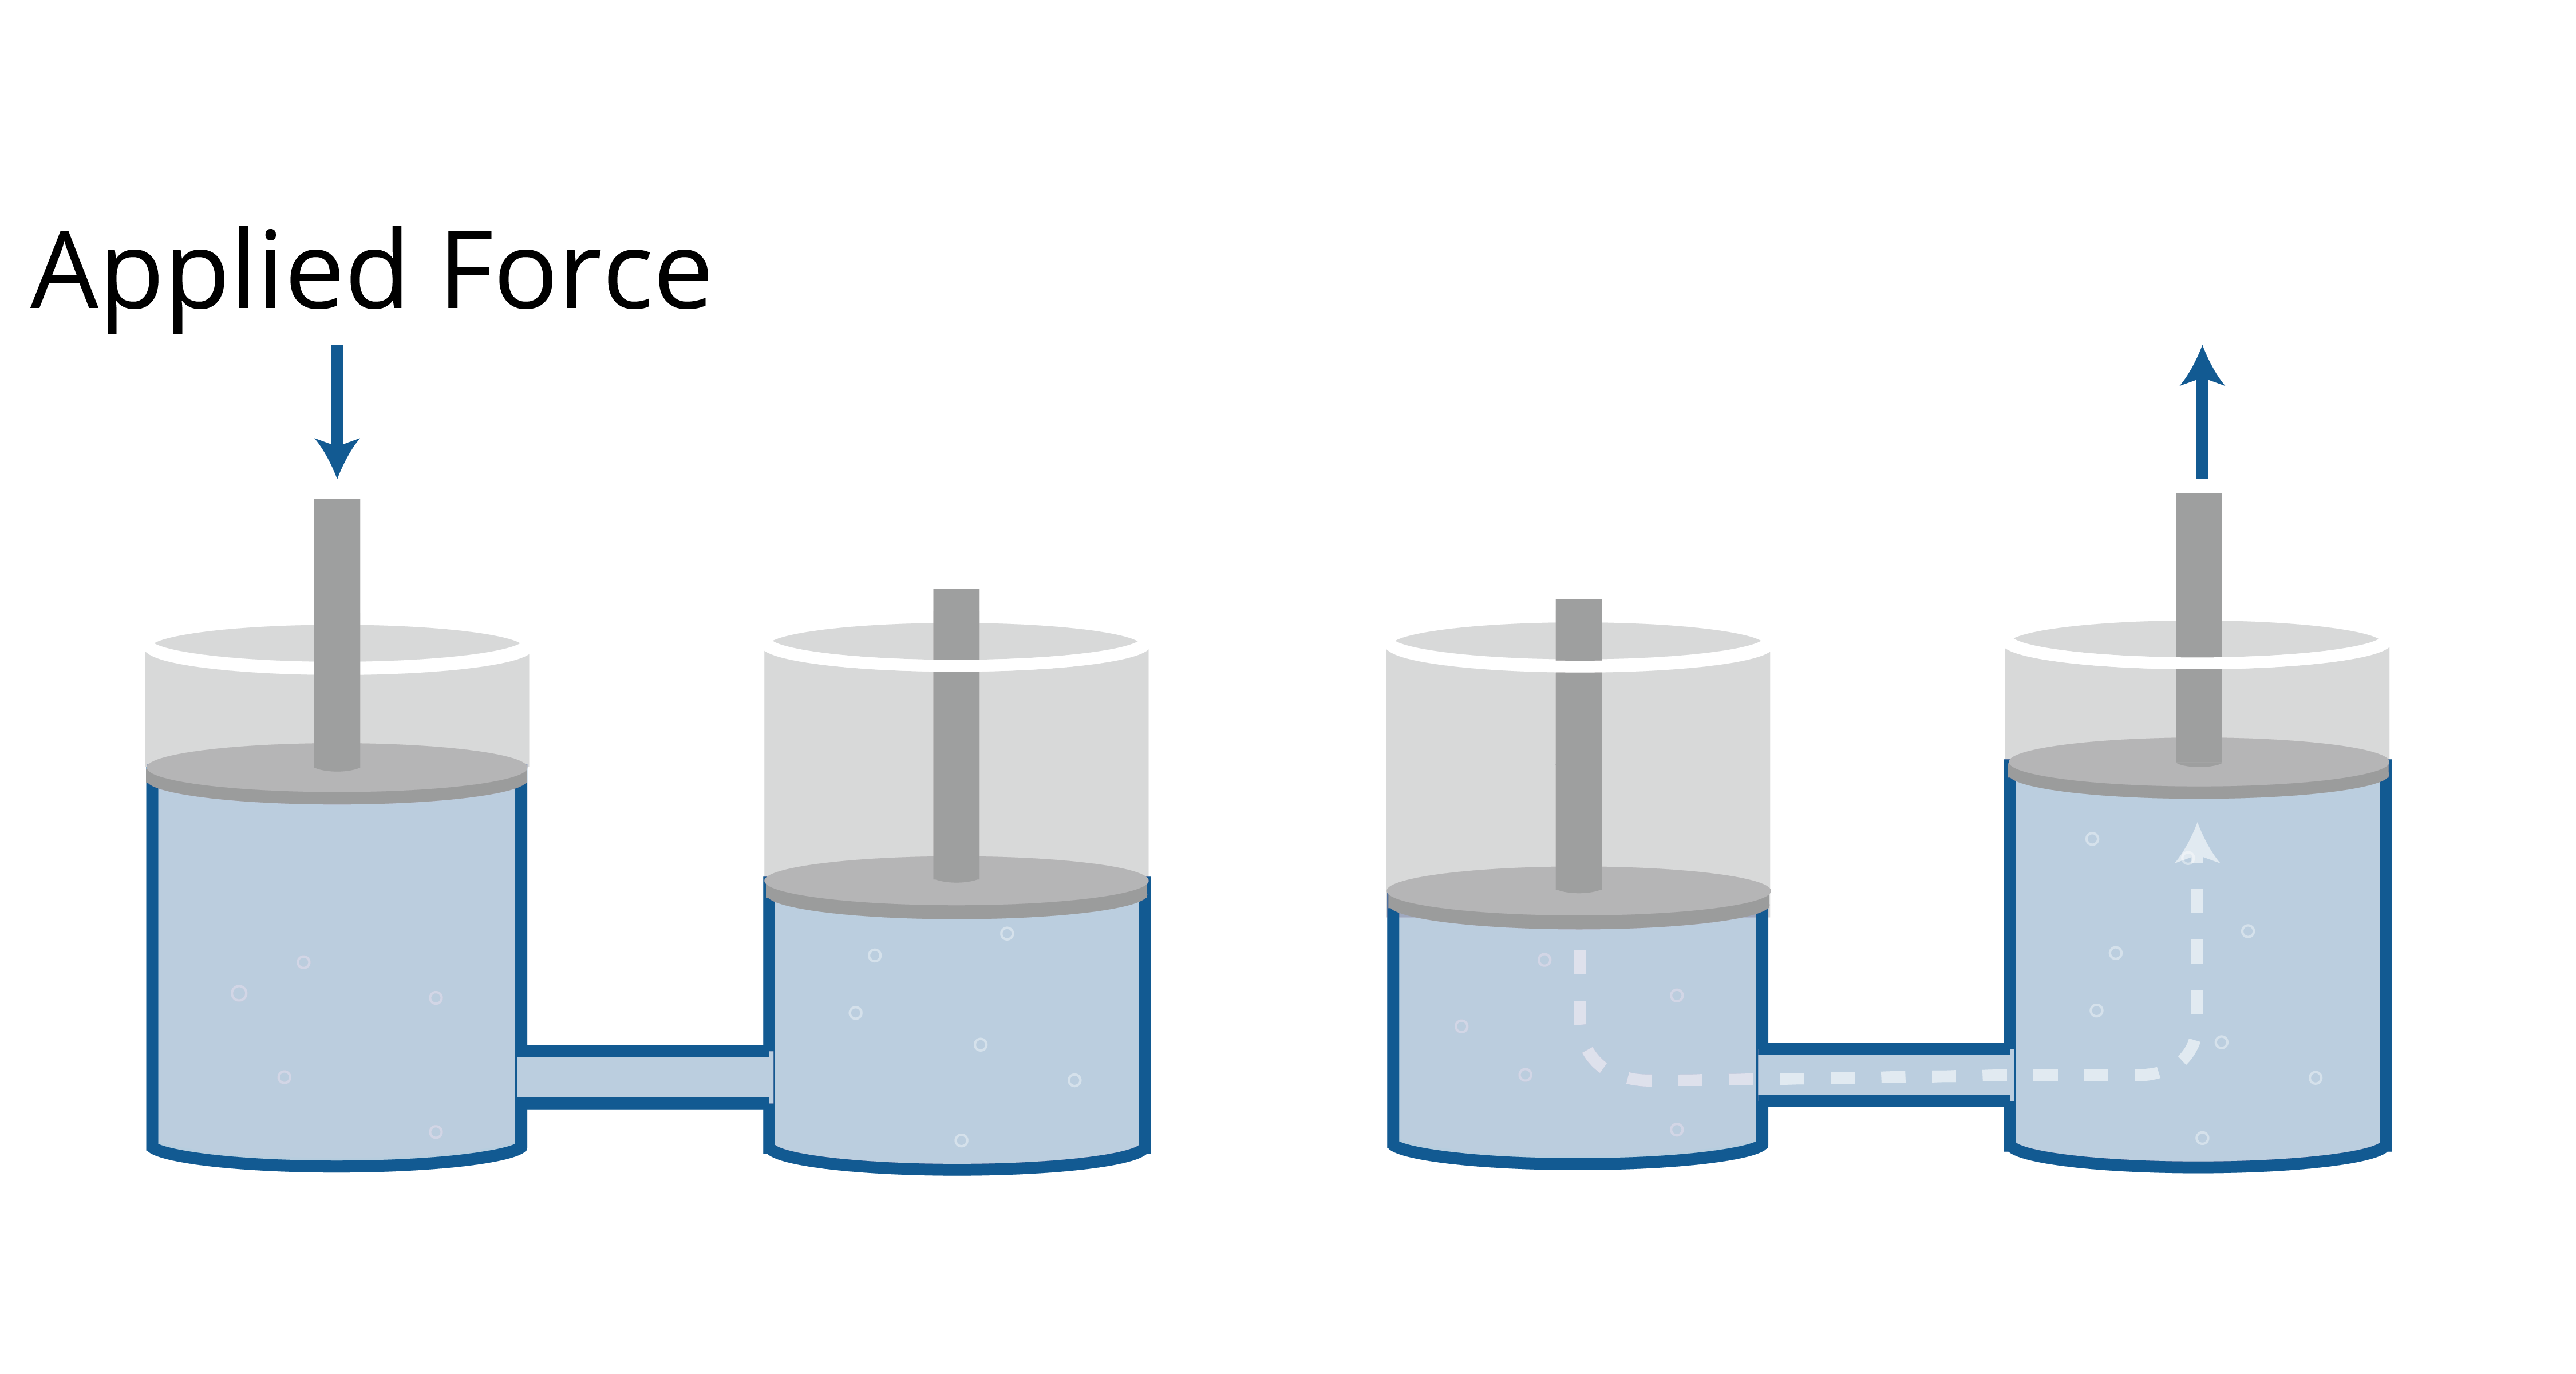
\includegraphics[width=\textwidth]{hydraulicsNew.png}

The pressure in the fluid is typically measured in pascals (Pa), which is equivalent to \(N / m^2\). We will use pascals for this calculation.

To calculate the pressure you create, divide the force applied by the area of the piston head. To determine the force on the other piston, multiply the pressure by the area of the second piston.

\begin{Exercise}[title={Hydraulics}, label=hydraulics]
Your car has disc brakes. When you apply 2,500,000 pascals of pressure to the brake fluid, the car stops quickly. As the car designer, you want this to require only 12 newtons of force from the driver's foot.

What should the radius of the master cylinder (the piston the driver pushes) be?
\end{Exercise}
\begin{Answer}[ref=hydraulics]
We are solving for the radius \( r \) of the piston. The area of the piston is \( \pi r^2 \), so the pressure is:

\[
\text{Pressure} = \frac{12}{\pi r^2}
\]

Setting the pressure equal to 2,500,000 pascals:

\[
2,500,000 = \frac{12}{\pi r^2}
\]

Solving for \( r \), we find:

\[
r = \sqrt{\frac{12}{\pi \times 2.5 \times 10^6}} \approx 0.00124 \text{ meters}.
\]
\end{Answer}
